\documentclass{report}

\usepackage[utf8]{inputenc}

\usepackage{Sweave}
\begin{document}
\Sconcordance{concordance:rapport_latex.tex:rapport_latex.Rnw:%
1 4 1 1 0 25 1 1 9 19 1 1 4 3 1 1 4 4 1 1 4 111 0 1 2 15 1 1 4 18 0 1 2 %
13 1 1 5 10 1 1 4 25 0 1 3 1 0 1 2 1 7 1 2 10 1 1 29 1 2 5 1 1 5 1 2 8 %
1}


\begin{titlepage}
    \begin{center}
        \vspace*{1cm}
 
        \Huge
        \textbf{Machine learning - DTU}
 
        \vspace{0.5cm}
        \LARGE
        Rapport 
 
        \vspace{1.5cm}
 
        \textbf{Anna Louise Hansen}
        \vfill
 
        Fra Udviklings- og Forenklingsstyrrelsen
 
        \vspace{0.8cm}
 
    \end{center}
\end{titlepage}



\chapter{Part I}

\section{Beskrivelse af data}
Alle boligejere i Danmark betaler en skat, ejendomsværdiskat, som er baseret på værdien af deres ejendom. Dette vil sige hele ejendommen inkl. grunden som boligen ligger på. For at kunne gøre dette laver den danske stat offentlige ejendomsvurderinger som disse skatter bliver baseret på. 
Det er derfor vigtigt at disse vurderinger er retvisende og ikke mindst forklarbare, således at en borger kan forstå hvilke parametre der ligger til grund for ejendomsvurderingen. 
Til dette project har jeg valgt at arbejde med anonymiseret data fra mit arbejde i udviklings- og forenklingsstyrrelsen, hvor jeg til dagligt arbejder med netop dette. Datasættet består af ejendomssalg fra en 6 årig periode. Ud over selve huspriserne består data også af en lang række attributter som beskriver karakteristika ved selve boligen. Det kan f.eks. være tagmateriale, boligens opførelsesår, information om størrelsen af huset og grunden eller bbr koder som dækker over boligens anvendelse. 
Der ud over består data også af en lang række attributter som fortæller noget om hvor boligens beliggenhed. Det kan f.eks. være boligens koordinater eller information om afstanden til kyst og skov eller afstand til motorvej og jernbane. 
Data kommer fra en række forskellige registre og offentlige styrrelser som eks. BBR og Styrrelsen for Dataforsyning og Effektivisering.

Til dette projekt vil jeg overordnet set prøve at se hvor godt man kan forudsige ejendomsværdier ud fra salgspriserne fra en 6-årig periode. 

Jeg vil med Principal Component Analysis få et overblik over de data der er til rådighed og få et visuelt overblik over attributterne. 
Herefter vil jeg med en unsupervised learning forsøge at gruppere det data jeg har til at generer yderlige attributer som kan indgå i modellen. Jeg vil her specifikt prøve at se om det er muligt at gruppere salgene i forskellige boligtyper. Jeg vil i samme omgang også forsøge at frasorterer outliers i data med anomaly detection. 
Herefter vil jeg med regressions model forsøge at kaste lys over projektets overordnede problem ved at forsøge at forudsige huspriserne ud fra salgspriser. I tilfælde af at modellen ikke ikke kan komme med en god prædiktion af en given ejendom vil det være muligt at denne ejendom bliver manuelt værdiansat af en sagsbehandler. Jeg vil derfor til slut med en classifikation forsøge at estimerer om en ejendom skal ud til manuel sagsbehandling baseret på dens estimerede ejendomsværdi.


\section{Detaljeret beskrivelse af data}



Det salgsdata som jeg har valgt at arbejde med dækker i udgangspunktet `r nrow(train)` observationer med `r ncol(train)` attributter. Inden jeg går i gang med at kigge på data har jeg valgt at lave en oprydning i data. Det har jeg gjort fordi mange af attributterne bliver i mit daglige arbejde brugt i forbindelse med imødekomme diverse forretningskrav. Desuden dækker observationerne mange forskellige typer af ejendomssalg. Det er en blanding af parcelhussalg, rækkehussalg, sommerhussalg, salg af ejerlejligheder mm. og ud fra et forretningsmæssigt perspektiv giver det ikke mening at træne en model på alle salg og ejendomstypen vil påvirke salgsprisen. F.eks. vil der på sommerhuse være restriktioner på hvor meget om året man må bo i sommerhuset og der kan være i sommerhusområder være andre regler for hvad man må bruge sin grund til end der er i et parcelhusområde. Jeg har derfor ligeledes valgt at reducerer antallet af observationer således at de kun dækker almindelige parcelhus. Dette er gjort ved kun at beholde alle de ejendomssalg, hvor ejendommen i BBR er registreret med enheds- og bygningsanvendelsen 120. 


Herefter er der `r nrow(train)` observationer tilbage og `r ncol(train)` attributter.

Der er for en del af attributterne en stor andel af manglende værdier. Det er især i forhold til variable fra BBR, som beskriver forskellige karakteristika ved selve boligen. Her har jeg har valgt at fjerne alle de attributter som har mere end 95\% manglende værdier.

\begin{Schunk}
\begin{Soutput}
|    |attributes                                                    |descrete_continous |attribute_type |attribute_class | missing_values| pct_missing_values|
|:---|:-------------------------------------------------------------|:------------------|:--------------|:---------------|--------------:|------------------:|
|72  |aux.adresse.etage                                             |descrete           |nomial         |character       |         241643|        100.0000000|
|99  |enhed.supplerendevarme                                        |descrete           |nomial         |character       |         241327|         99.8692286|
|98  |enhed.opvarmningsmiddel                                       |descrete           |nomial         |character       |         241100|         99.7752883|
|101 |enhed.varmeinstallation                                       |descrete           |nomial         |character       |         240651|         99.5894770|
|28  |aux.ice_info.adresse.afstand_mellem_soe                       |descrete           |ratio          |numeric         |         222433|         92.0502560|
|86  |bygning.afloebsforhold                                        |descrete           |nomial         |character       |         168597|         69.7711086|
|27  |aux.ice_info.adresse.afstand_lille_soe                        |descrete           |ratio          |numeric         |         137535|         56.9166084|
|89  |bygning.supplerendevarme                                      |descrete           |nomial         |character       |         133291|         55.1602985|
|95  |enhed.energiforsyning                                         |descrete           |nomial         |character       |         116534|         48.2256883|
|88  |bygning.opvarmningsmiddel                                     |descrete           |nomial         |character       |         112131|         46.4035788|
|105 |fremskreven_pris                                              |continous          |interval       |numeric         |           2913|          1.2054974|
|106 |fremskreven_pris_M2                                           |continous          |interval       |numeric         |           2913|          1.2054974|
|104 |aux.vurbenyttelseskode                                        |descrete           |nomial         |character       |            337|          0.1394619|
|34  |aux.ice_info.adresse.udsigtslinjer_hav                        |descrete           |ratio          |integer         |            293|          0.1212533|
|36  |aux.ice_info.adresse.udsigtslaengde_samlet                    |descrete           |ratio          |numeric         |            293|          0.1212533|
|37  |aux.ice_info.adresse.udsigtslinjer_soe                        |descrete           |ratio          |integer         |            293|          0.1212533|
|1   |aux.adresse.etrs89koordinatnord                               |descrete           |interval       |numeric         |            263|          0.1088382|
|2   |aux.adresse.etrs89koordinatoest                               |descrete           |interval       |numeric         |            263|          0.1088382|
|69  |EV_NN_M2                                                      |descrete           |interval       |numeric         |            263|          0.1088382|
|73  |aux.adresse.regionskode                                       |descrete           |nomial         |integer         |            263|          0.1088382|
|94  |enhed.badeforhold                                             |descrete           |nomial         |character       |             26|          0.0107597|
|100 |enhed.toiletforhold                                           |descrete           |nomial         |character       |             25|          0.0103458|
|92  |bygning.varmeinstallation                                     |descrete           |nomial         |character       |              9|          0.0037245|
|3   |aux.ice_info.adresse.afstand_kyst                             |descrete           |ratio          |numeric         |              0|          0.0000000|
|4   |aux.ice_info.adresse.afstand_lokalvej                         |descrete           |ratio          |numeric         |              0|          0.0000000|
|5   |aux.ice_info.adresse.afstand_trafikvej_fordeling              |descrete           |ratio          |numeric         |              0|          0.0000000|
|6   |aux.ice_info.adresse.afstand_trafikvej_gennemfart             |descrete           |ratio          |numeric         |              0|          0.0000000|
|7   |aux.ice_info.adresse.afstand_motorvej_motortrafikvej          |descrete           |ratio          |numeric         |              0|          0.0000000|
|8   |aux.ice_info.adresse.afstand_jernbane_hovedbane               |descrete           |ratio          |numeric         |              0|          0.0000000|
|9   |aux.ice_info.adresse.afstand_jernbane_any                     |descrete           |ratio          |numeric         |              0|          0.0000000|
|10  |aux.ice_info.adresse.afstand_jernbane_lokalbane               |descrete           |ratio          |numeric         |              0|          0.0000000|
|11  |aux.ice_info.adresse.afstand_jernbane_metro                   |descrete           |ratio          |numeric         |              0|          0.0000000|
|12  |aux.ice_info.adresse.afstand_jernbane_regionalbane            |descrete           |ratio          |numeric         |              0|          0.0000000|
|13  |aux.ice_info.adresse.afstand_jernbane_region_privat           |descrete           |ratio          |numeric         |              0|          0.0000000|
|14  |aux.ice_info.adresse.afstand_jernbane_s_bane                  |descrete           |ratio          |numeric         |              0|          0.0000000|
|15  |aux.ice_info.adresse.afstand_stor_skov                        |descrete           |ratio          |numeric         |              0|          0.0000000|
|16  |aux.ice_info.adresse.afstand_lille_skov                       |descrete           |ratio          |numeric         |              0|          0.0000000|
|17  |aux.ice_info.adresse.afstand_lokalnet_hoejspaending           |descrete           |ratio          |numeric         |              0|          0.0000000|
|18  |aux.ice_info.adresse.afstand_regionalnet_hoejspaending        |descrete           |ratio          |numeric         |              0|          0.0000000|
|19  |aux.ice_info.adresse.afstand_transmissionsnet_hoejspaending   |descrete           |ratio          |numeric         |              0|          0.0000000|
|20  |aux.ice_info.adresse.afstand_lille_vandloeb                   |descrete           |ratio          |numeric         |              0|          0.0000000|
|21  |aux.ice_info.adresse.afstand_mellem_vandloeb                  |descrete           |ratio          |numeric         |              0|          0.0000000|
|22  |aux.ice_info.adresse.afstand_stort_vandloeb                   |descrete           |ratio          |numeric         |              0|          0.0000000|
|23  |aux.ice_info.adresse.afstand_ukendt_vandloeb                  |descrete           |ratio          |numeric         |              0|          0.0000000|
|24  |aux.ice_info.adresse.afstand_station_metro                    |descrete           |ratio          |numeric         |              0|          0.0000000|
|25  |aux.ice_info.adresse.afstand_station_s_tog                    |descrete           |ratio          |numeric         |              0|          0.0000000|
|26  |aux.ice_info.adresse.afstand_station_tog                      |descrete           |ratio          |numeric         |              0|          0.0000000|
|29  |aux.ice_info.adresse.afstand_stor_soe                         |descrete           |ratio          |numeric         |              0|          0.0000000|
|30  |aux.ice_info.adresse.afstand_lille_vindmoelle                 |descrete           |ratio          |numeric         |              0|          0.0000000|
|31  |aux.ice_info.adresse.afstand_mellem_vindmoelle                |descrete           |ratio          |numeric         |              0|          0.0000000|
|32  |aux.ice_info.adresse.afstand_stor_vindmoelle                  |descrete           |ratio          |numeric         |              0|          0.0000000|
|33  |aux.ice_info.adresse.areal_samlet_skov                        |descrete           |ratio          |numeric         |              0|          0.0000000|
|35  |aux.ice_info.adresse.udsigtslaengde_hav                       |descrete           |ratio          |numeric         |              0|          0.0000000|
|38  |aux.ice_info.adresse.udsigtslaengde_soe                       |descrete           |ratio          |numeric         |              0|          0.0000000|
|39  |aux.ice_info.bygning.etager.arealaflovligbeboelseikaelder     |descrete           |ratio          |integer         |              0|          0.0000000|
|40  |aux.ice_info.bygning.etager.arealafudnyttetdelaftagetage      |descrete           |ratio          |integer         |              0|          0.0000000|
|41  |aux.ice_info.bygning.etager.etagensadgangsareal               |descrete           |ratio          |integer         |              0|          0.0000000|
|42  |aux.ice_info.bygning.etager.kaelderareal                      |descrete           |ratio          |integer         |              0|          0.0000000|
|43  |aux.ice_info.bygning.etager.samletarealaftagetage             |descrete           |ratio          |integer         |              0|          0.0000000|
|44  |aux.ice_info.byzoneareal_opsummeret_delj                      |descrete           |ratio          |integer         |              0|          0.0000000|
|45  |aux.ice_info.landzoneareal_opsummeret_delj                    |descrete           |ratio          |integer         |              0|          0.0000000|
|46  |aux.ice_info.sommerhuszoneareal_opsummeret_delj               |descrete           |ratio          |integer         |              0|          0.0000000|
|47  |aux.ice_info.jordstykker.registreretareal_fratrukket_vejareal |descrete           |ratio          |integer         |              0|          0.0000000|
|48  |aux.ice_info.jordstykker.vejareal                             |descrete           |ratio          |integer         |              0|          0.0000000|
|49  |bolig_alder                                                   |descrete           |ratio          |integer         |              0|          0.0000000|
|50  |bolig_areal                                                   |descrete           |ratio          |numeric         |              0|          0.0000000|
|51  |bygning.antaletager                                           |descrete           |interval       |integer         |              0|          0.0000000|
|52  |bygning.arealindbyggetcarport                                 |descrete           |ratio          |integer         |              0|          0.0000000|
|53  |bygning.arealindbyggetgarage                                  |descrete           |ratio          |integer         |              0|          0.0000000|
|54  |bygning.bebyggetareal                                         |descrete           |ratio          |integer         |              0|          0.0000000|
|55  |bygning.bygningenssamledeboligareal                           |descrete           |ratio          |integer         |              0|          0.0000000|
|56  |bygning.bygningenssamledeerhvervsareal                        |descrete           |ratio          |integer         |              0|          0.0000000|
|57  |bygning.omtilbygningsaar                                      |descrete           |interval       |integer         |              0|          0.0000000|
|58  |bygning.opfoerelsesaar                                        |descrete           |interval       |integer         |              0|          0.0000000|
|59  |bygning.samletbygningsareal                                   |descrete           |ratio          |integer         |              0|          0.0000000|
|60  |enhed.antalbadevaerelser                                      |descrete           |ratio          |integer         |              0|          0.0000000|
|61  |enhed.antalvaerelser                                          |descrete           |ratio          |integer         |              0|          0.0000000|
|62  |enhed.antalvandskylledetoiletter                              |descrete           |ratio          |integer         |              0|          0.0000000|
|63  |enhed.arealtilbeboelse                                        |descrete           |ratio          |integer         |              0|          0.0000000|
|64  |enhed.arealtilerhverv                                         |descrete           |ratio          |integer         |              0|          0.0000000|
|65  |enhed.enhedenssamledeareal                                    |descrete           |ratio          |integer         |              0|          0.0000000|
|66  |etage.arealafudnyttetdelaftagetage                            |descrete           |ratio          |integer         |              0|          0.0000000|
|67  |etage.etagensadgangsareal                                     |descrete           |ratio          |integer         |              0|          0.0000000|
|68  |etage.kaelderareal                                            |descrete           |ratio          |integer         |              0|          0.0000000|
|70  |ice_info.min_koteletratiobuff250                              |continous          |interval       |numeric         |              0|          0.0000000|
|71  |ombyg_alder                                                   |descrete           |interval       |numeric         |              0|          0.0000000|
|74  |aux.ice_info.bb_anvendelse_0                                  |descrete           |ratio          |integer         |              0|          0.0000000|
|75  |aux.ice_info.bb_anvendelse_910                                |descrete           |ratio          |integer         |              0|          0.0000000|
|76  |aux.ice_info.bb_anvendelse_920                                |descrete           |ratio          |integer         |              0|          0.0000000|
|77  |aux.ice_info.bb_anvendelse_930                                |descrete           |ratio          |integer         |              0|          0.0000000|
|78  |aux.ice_info.bb_anvendelse_940                                |descrete           |ratio          |integer         |              0|          0.0000000|
|79  |aux.ice_info.bb_anvendelse_950                                |descrete           |ratio          |integer         |              0|          0.0000000|
|80  |aux.ice_info.bb_anvendelse_960                                |descrete           |ratio          |integer         |              0|          0.0000000|
|81  |aux.ice_info.bb_anvendelse_970                                |descrete           |ratio          |integer         |              0|          0.0000000|
|82  |ice_info.bb_per_delgrund                                      |descrete           |ratio          |integer         |              0|          0.0000000|
|83  |ice_info.en_per_delgrund                                      |descrete           |ratio          |integer         |              0|          0.0000000|
|84  |ice_info.et_per_delgrund                                      |descrete           |ratio          |integer         |              0|          0.0000000|
|85  |ice_info.js_per_delgrund                                      |descrete           |ratio          |integer         |              0|          0.0000000|
|87  |bygning.bygningensanvendelse                                  |descrete           |nomial         |integer         |              0|          0.0000000|
|90  |bygning.tagdaekningsmateriale                                 |descrete           |nomial         |character       |              0|          0.0000000|
|91  |bygning.vandforsyning                                         |descrete           |nomial         |integer         |              0|          0.0000000|
|93  |bygning.ydervaeggensmateriale                                 |descrete           |nomial         |character       |              0|          0.0000000|
|96  |enhed.enhedensanvendelse                                      |descrete           |nomial         |integer         |              0|          0.0000000|
|97  |enhed.koekkenforhold                                          |descrete           |nomial         |character       |              0|          0.0000000|
|102 |etage.bygningensetagebetegnelse                               |descrete           |nomial         |character       |              0|          0.0000000|
|103 |region_nr                                                     |descrete           |nomial         |integer         |              0|          0.0000000|
\end{Soutput}
\end{Schunk}

Som udgangspunkt vil jeg træne en model som skal være i stand til at kunne prædiktere værdien af et standard
parcelhus. Data som der skal trænes på skal derfor også være salg af standard parcelhuse.
Data er derfor blevet ensrettet på følgende måde:

% - enhed.antalvaerelser > 1 og enhed.antalvaerelser < 10
% - bolig_areal < 500 og bolig_areal > 50
% - bolig_alder > 0 og bolig_alder < 100
% - bygning.antaletager > 0 og bygning.antaletager < 4
% - enhed.antalbadevaerelser > 0 og enhed.antalbadevaerelser < 4
% - enhed.antalvandskylledetoiletter > 0 og enhed.antalvandskylledetoiletter < 4
% - fremskreven_pris_M2 < 30000 og fremskreven_pris_M2 > 0

Slutteligt er der blevet taget et valg om kun at udvælge de rå attributter som menes at være de
vigtigste i forhold til at forudsige værdien af et standad parcelhus.

\begin{Schunk}
\begin{Soutput}
|attributes                                                    |descrete_continous |attribute_type |attribute_class | missing_values| pct_missing_values|
|:-------------------------------------------------------------|:------------------|:--------------|:---------------|--------------:|------------------:|
|fremskreven_pris_M2                                           |continous          |interval       |numeric         |              0|                  0|
|bygning.ydervaeggensmateriale                                 |descrete           |nomial         |character       |              0|                  0|
|bygning.tagdaekningsmateriale                                 |descrete           |nomial         |character       |              0|                  0|
|ombyg_alder                                                   |descrete           |interval       |numeric         |              0|                  0|
|enhed.antalvaerelser                                          |descrete           |ratio          |integer         |              0|                  0|
|enhed.antalbadevaerelser                                      |descrete           |ratio          |integer         |              0|                  0|
|enhed.antalvandskylledetoiletter                              |descrete           |ratio          |integer         |              0|                  0|
|bolig_areal                                                   |descrete           |ratio          |numeric         |              0|                  0|
|bolig_alder                                                   |descrete           |ratio          |integer         |              0|                  0|
|aux.ice_info.jordstykker.registreretareal_fratrukket_vejareal |descrete           |ratio          |integer         |              0|                  0|
|aux.ice_info.adresse.afstand_motorvej_motortrafikvej          |descrete           |ratio          |numeric         |              0|                  0|
|aux.ice_info.adresse.afstand_kyst                             |descrete           |ratio          |numeric         |              0|                  0|
|EV_NN_M2                                                      |descrete           |interval       |numeric         |              0|                  0|
\end{Soutput}
\end{Schunk}

 
De to attributter der dækker over tagtypematriale og ydervægsmateriale er diskrete variable som fordel
kan normaliseres med en one-out-of-k transformering.

Afstand til kyst og afstand til motorvej er to variable som jeg har valgt at binariserer. Det har jeg da de to
features forud for denne rapport er blevet imputeret. For afstand til kyst er afstanden op til 1500 meter målt.
Alt herover er imputeret til 1501 meter. Ligeledes er gjort for afstand til motorvej.
For at håndtere disse variable har jeg som sagt valgt at binariserer dem. For afstand til kyst har jeg ud fra et
forretningsmæssigt synspunkt valgt at en ejendom ligger så tæt på kysten at det har en effekt i dens værdi hvis
den ligger inden for 300 meter af kysten. Det samme er gjort for afstand til vej. Her er grænsen dog blot 100
meter.



\section{Data visualisering heriblandt Principal Component Analysis (PCA)}

De forskellige attributter indeholder ikke værdier på samme skala og jeg har derfor valgt at standardisere data.
Selve standardiseringen betyder at data for hver attribut reskaleres således at det får et gennemsnit på 1 med en
standardafvigelse på 1.

% $(X-\mu)/sd$ 
% 
Efter at have standardiseret data laves der en correlationsanalyse hvor resultaterne af visualiseres i et correlationsplot.

\begin{Schunk}
\begin{Soutput}
 [1] "fremskreven_pris_M2"                                          
 [2] "ombyg_alder"                                                  
 [3] "enhed.antalvaerelser"                                         
 [4] "enhed.antalbadevaerelser"                                     
 [5] "enhed.antalvandskylledetoiletter"                             
 [6] "bolig_areal"                                                  
 [7] "bolig_alder"                                                  
 [8] "aux.ice_info.jordstykker.registreretareal_fratrukket_vejareal"
 [9] "EV_NN_M2"                                                     
[10] "ydervaegsmateriale_mursten"                                   
[11] "ydervaegsmateriale_gasbeton"                                  
[12] "ydervaegsmateriale_bindingsvaerk"                             
[13] "ydervaegsmateriale_traebeklaedning"                           
[14] "ydervaegsmateriale_andet"                                     
[15] "tagtype_builtup"                                              
[16] "tagtype_tagpap"                                               
[17] "tagtype_fibercement"                                          
[18] "tagtype_cementsten"                                           
[19] "tagtype_tegl"                                                 
[20] "tagtype_straatag"                                             
[21] "tagtype_andet"                                                
[22] "taet_paa_kyst"                                                
[23] "taet_paa_motorvej"                                            
\end{Soutput}
\end{Schunk}
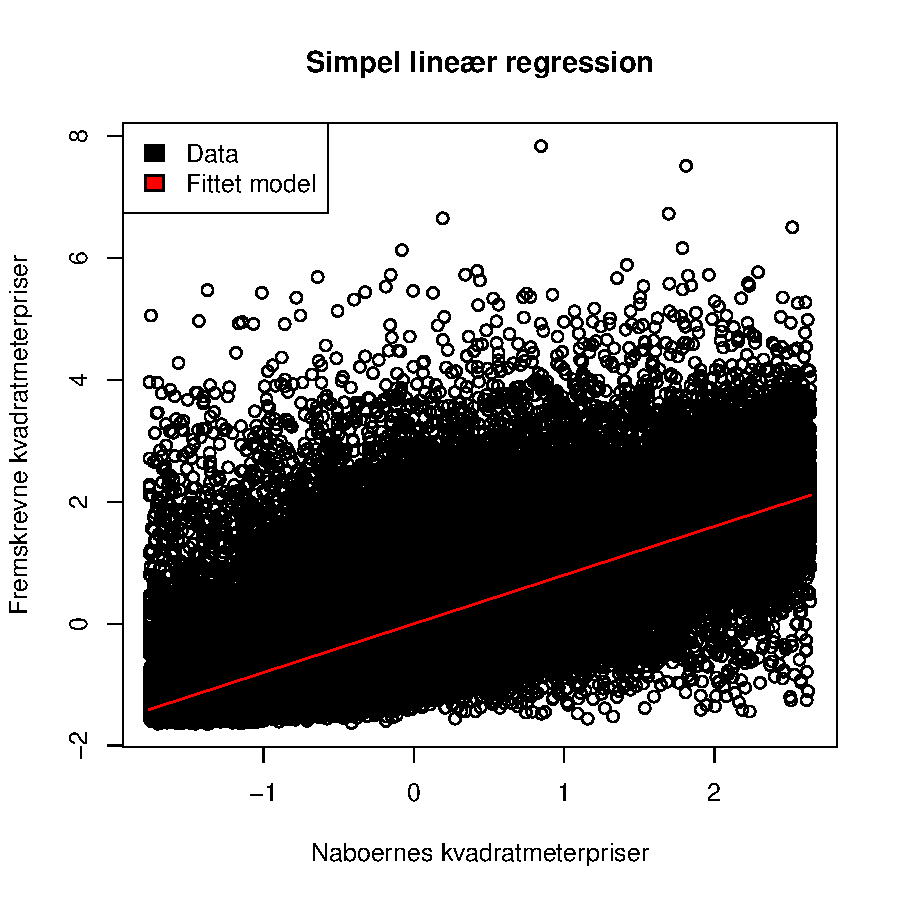
\includegraphics{rapport_latex-007}

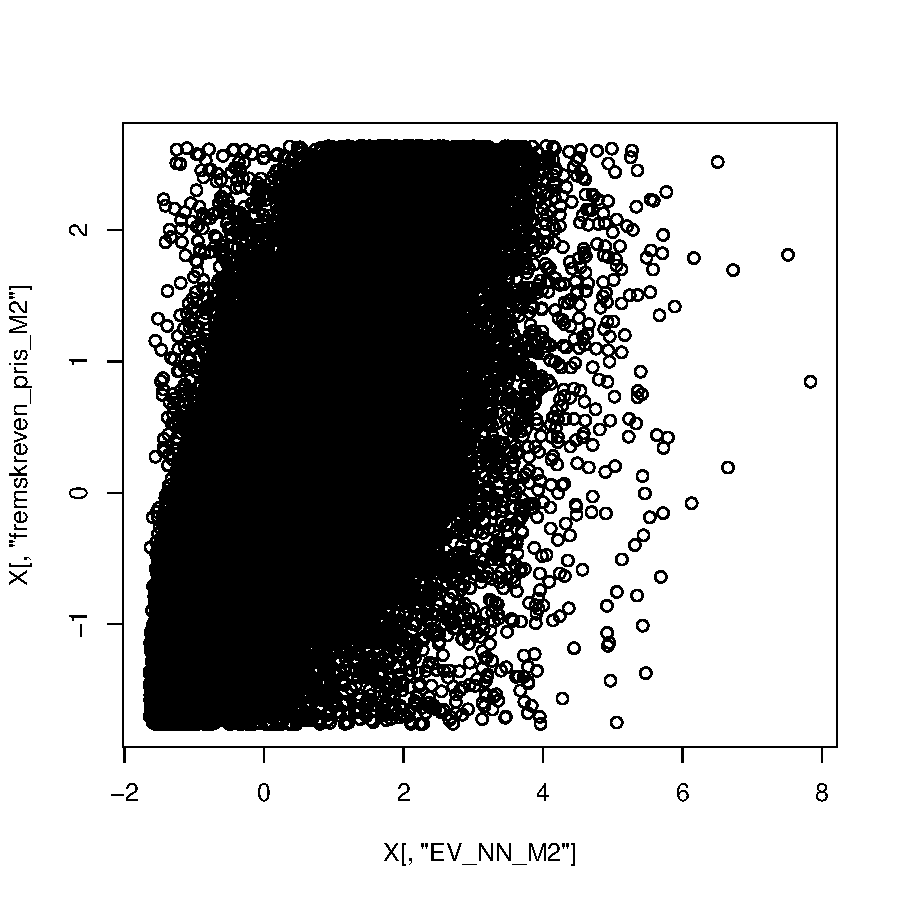
\includegraphics{rapport_latex-008}


Salgsdata består efter alle datatransformationerne af `r N` observationer (N) med `r M` features (M).
En af de stærkere correlerede variable i data er EV\_NN\_M2 og de fremskrevne handelspriser. EV\_NN\_M2 er en variabel som dækker over områdeprisen. Den dækker over et vægtet gennemsnit over de nærmeste 15 solgte naboers kvadratmeterpriser. Det giver altså rigtig god mening at der er en stor korrelation mellem de solgte naboers kvadratmeter priser og ejendommens egen kvadratmeterpris.
Når de to variable plottes mod hinanden ser det således ud:

Der er en stærk korrelation mellem naboernes kvadratmeterpriser og ejendommens egen kvadratmeterpris. Det er fordi at priserne for en given lokation i høj grad er med til at bestemme prisen for en ejendom.
Udover områdeprisen er det boligens egen karakteristika som er med til at udgøre den samlede ejendomsværdi.

Som en del af PCA udregnes herefter Singular Value Decomposition (SVD).

\includegraphics{rapport_latex-009}

De foeste 16 principal components kan man forklare 90\% af variationen i data. For at kommme over 95\% skal man have de 18 foerste komponenter. Der er i alt 23 mulige komponenter.
Det som det umiddelbart synes at betyde er at der ikke kan reduceres mange attibutter væk uden at det betyder at man mister variation.
PCA analysen kan bruges til at visualiserer data, feature extraction og compression.
Principal component analyse kan bruges til at reducerer dementionerne i data.

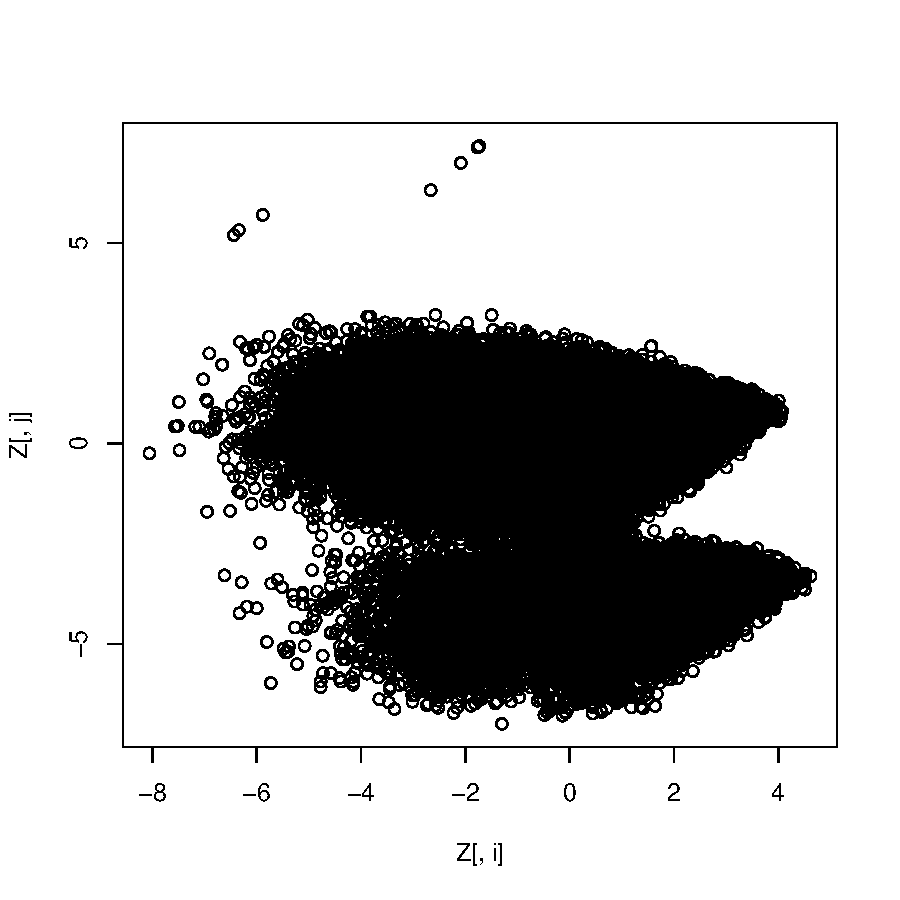
\includegraphics{rapport_latex-010}


\chapter{Part II}

I denne første del af del2 vil jeg med en linear regression forsøge at forudsige handelspriser baseret på bl.a. områdeprisen. Da der er en klar sammenhæng mellem hvad en ejendom bliver solgt for og hvad naboerne i området bliver solgt for er det klart en variabel som skal indgå i den lineære regressions model. Desuden er størrelsen og standen på ejendommen også relevant. Jeg har ikke stand som en attribut i mit datasæt men vil i stedet bruge boligens opførelsesår og ombygningsår som et inddirekte mål for dette. Er ejendommen eks. opført i starten af 1900 men har siden ingen ombygninger haft vil det i langt de fleste tilfælde betyde at bygningen er i en dårligere stand end en ejendom opført i 1970 med en ombygning i 2010. Det er kun større ombygninger som registreres i BBR. 
Håbet med denne regressionsanalyse er at man ud fra relativt få variable og en relativt simpel model vil kunne forudsige ejendomspriserne. Årsagen til at dette er en interessant analyse er at der med de tidligere offentlige ejendomsvurderinger har været store problemer i forhold til at forklare den enkelte borger hvorfor vedkommenes ejendomsværdi er som den er. 

Forud for regressionsanalysen er data blevet tranformeret. For faktorvariablene tagtype og vægmateriale har jeg valgt at tranformere med en one-of-k transformering. Herefter er alle attributer blevet standardiseret, således at de har en gennemsnit på 0 og en standardafvigelse på 1. 

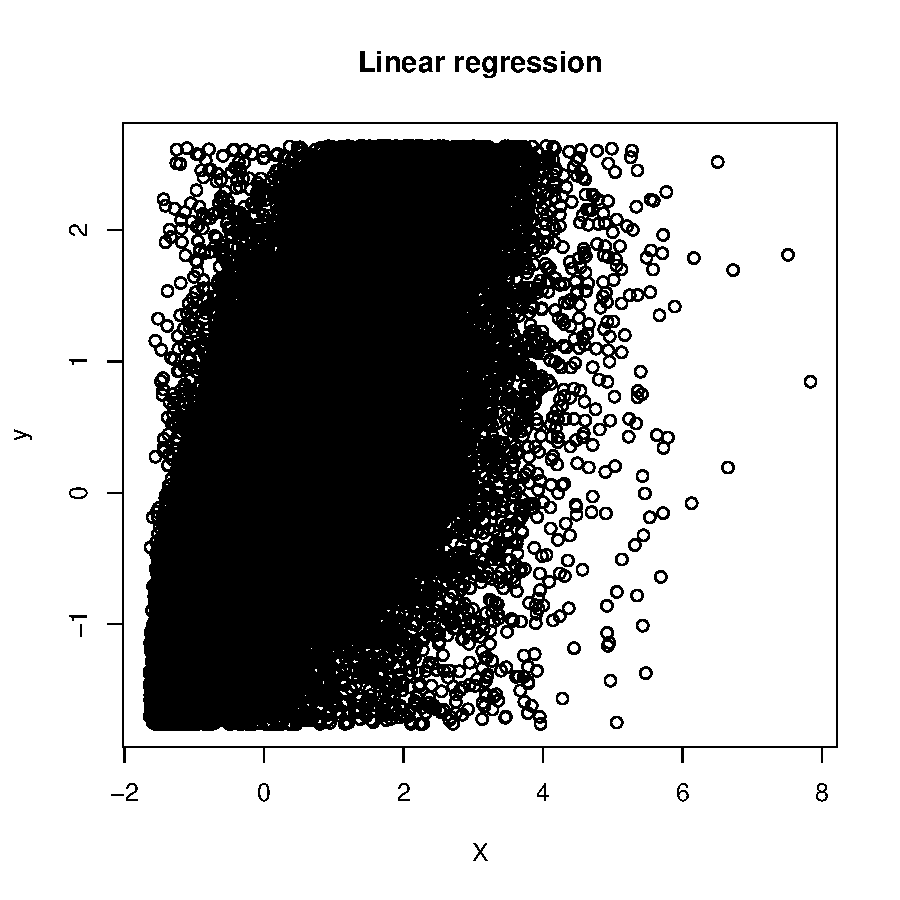
\includegraphics{rapport_latex-011}

Til at estimere modelparametrene til den lineære regressionsmodel har jeg den fremskrevne handelspris som den afhængige variabel og nabopriserne som prediktorvariabel. 

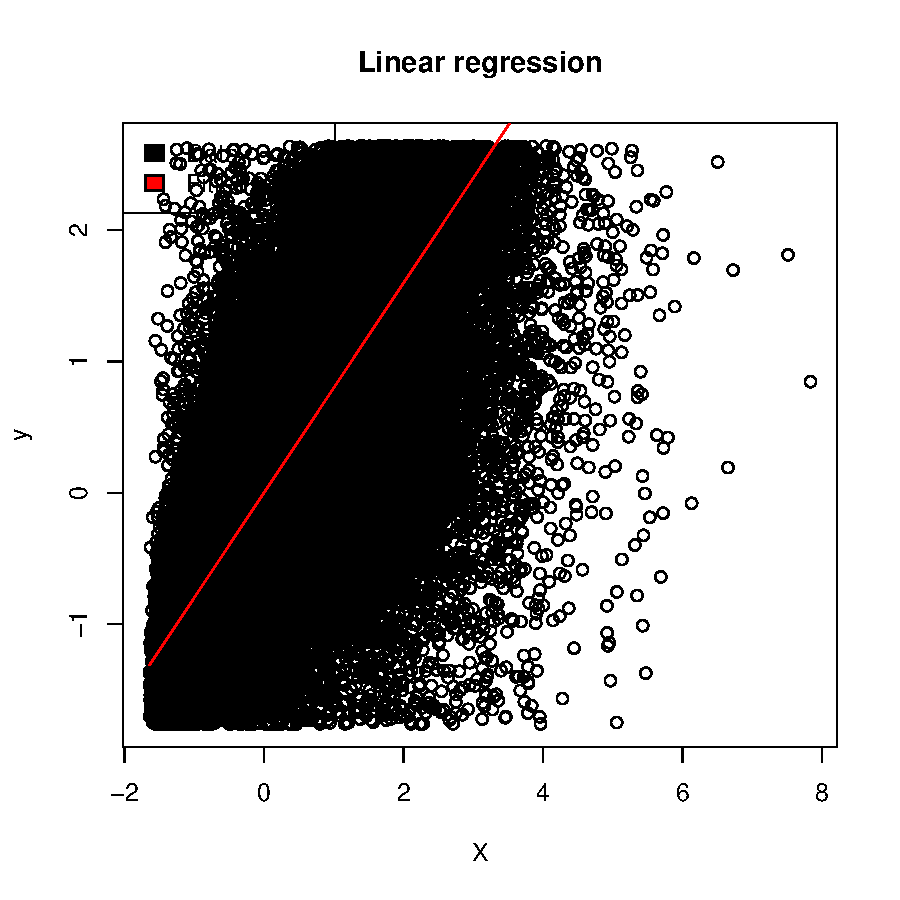
\includegraphics{rapport_latex-012}

Evalueringen af den lineære model kan foregå ved at man træner på et datasæt og prædikterer på et andet. I følgende regression har jeg nabokvadratmeterpriserne og boligarealet med som prediktorvariable. 

\begin{Schunk}
\begin{Soutput}
y ~ X1 + X2
\end{Soutput}
\end{Schunk}
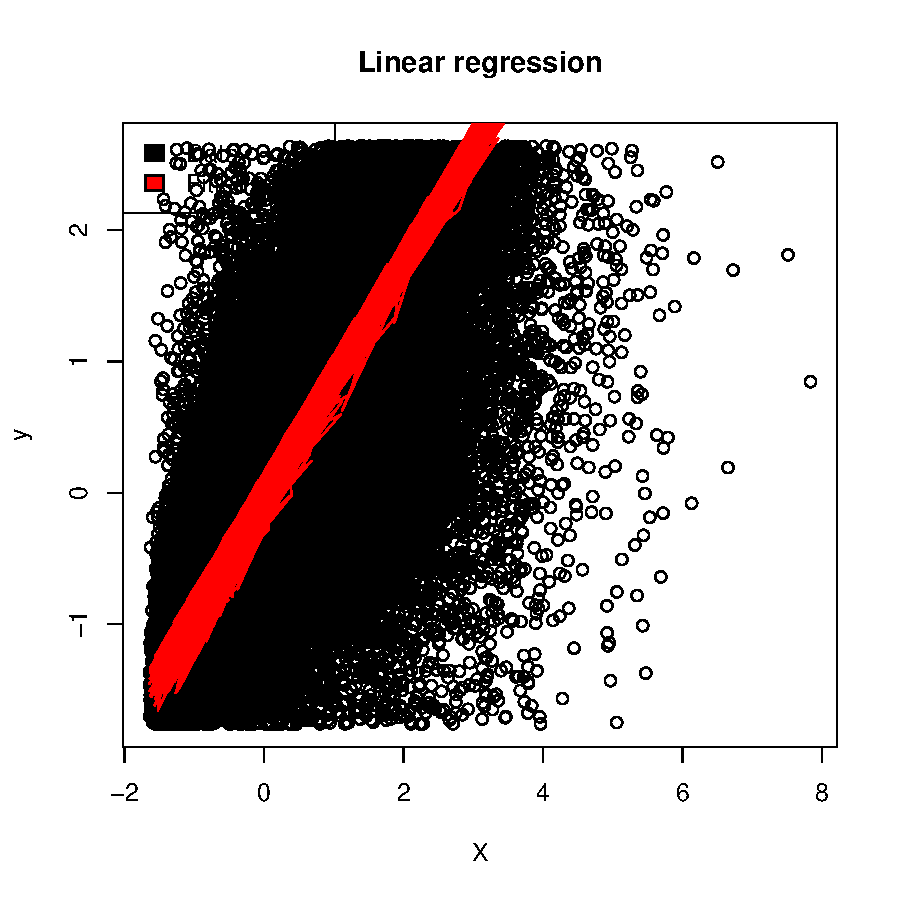
\includegraphics{rapport_latex-013}

Ud fra den estimerede model kan man plotte sin afhængige variabel mod de predikterede værdier.
Forskellen mellem den faktiske afhænge variabel (i dette tilfælde de fremskrevne salgspiser) og den prædikterede variabel (modellens estimerede y) er residualet.

\begin{Schunk}
\begin{Soutput}
y ~ EV_NN_M2 + bolig_areal
\end{Soutput}
\begin{Soutput}
Call:
lm(formula = fmla, data = Xr)

Residuals:
    Min      1Q  Median      3Q     Max 
-5.8248 -0.3216  0.0218  0.3579  3.6482 

Coefficients:
              Estimate Std. Error t value Pr(>|t|)    
(Intercept)  3.491e-15  1.389e-03    0.00        1    
EV_NN_M2     8.054e-01  1.395e-03  577.52   <2e-16 ***
bolig_areal -7.184e-02  1.395e-03  -51.52   <2e-16 ***
---
Signif. codes:  0 '***' 0.001 '**' 0.01 '*' 0.05 '.' 0.1 ' ' 1

Residual standard error: 0.5973 on 185015 degrees of freedom
Multiple R-squared:  0.6432,	Adjusted R-squared:  0.6432 
F-statistic: 1.668e+05 on 2 and 185015 DF,  p-value: < 2.2e-16
\end{Soutput}
\end{Schunk}
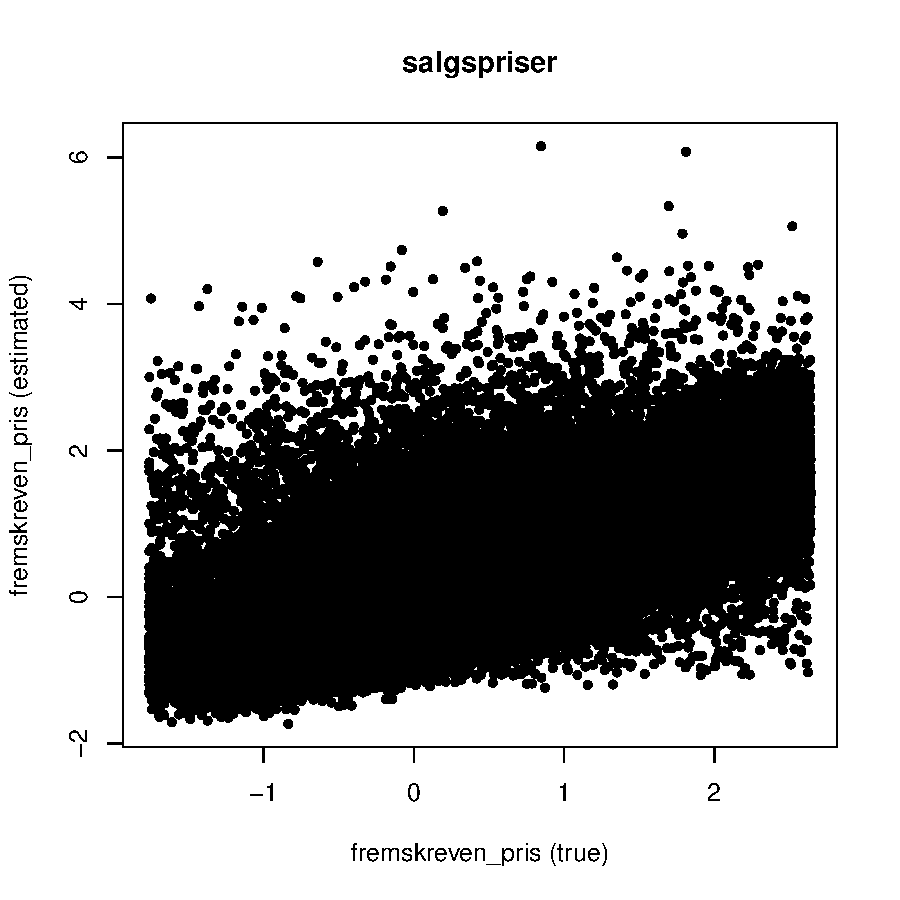
\includegraphics{rapport_latex-014}


2. Introduce a regularization parameter <U+03BB> as discussed in chapter 14 of the lecture
notes, and estimate the generalization error for different values of <U+03BB>. Specifically, choose a reasonable range of values of <U+03BB> (ideally one where the generalization error first drop and then increases), and for each value use K = 10
fold cross-validation (algorithm 5) to estimate the generalization error.
Include a figure of the estimated generalization error as a function of <U+03BB> in the
report and briefly discuss the result.
3. Explain how a new data observation is predicted according to the linear model
with the lowest generalization error as estimated in the previous question.
I.e., what are the effects of the selected attributes in terms of determining the
predicted class. Does the result make sense?


\chapter{Part III}


\end{document}
